\documentclass[man,natbib]{apa6}

\title{Personal statement on learning and instruction}
\shorttitle{Learning and instruction}
\author{Colby Goettel}
\affiliation{Brigham Young University}

\usepackage{graphicx}

\newcommand\vref[3]{(#1~#2\thinspace:\thinspace#3)}

\abstract{David Kolb defined learning as ``the process whereby knowledge is created through the transformation of experience'' \citep{kolb2014experiential}. Learning is an experienced activity. Knowledge can be carried to the learner, but the learner must choose to work and rework that knowledge until it has become a part of them. This internalization is how knowledge is created: the learner must construct it once it has been brought to them. Simply transmitting knowledge is not enough to cause learning to happen.}

\begin{document}
\maketitle

% The purpose of learning
The purpose of learning is to grow as an individual. To grow as a society. To better mankind. Everything we do, or everything we ought to do, is to better mankind. As a student, my purpose for learning is to better mankind. There's a reason BYU's motto ends ``go forth to serve.'' As a disciple, my purpose is to ``first seek to obtain [the Lord's] word'' \vref{D\&C}{11}{21}~--- to learn~--- and \emph{then} to apply it and better myself and better mankind.

Even as a Linux system administrator, my purpose is to better mankind. This is why open source software and documentation are so important: the one is able to benefit the many. For information technology (IT) professionals, everything we need to know is online. We built the Internet and put everything we know on it. At this point, there will probably only be one or two problems in my career that no one else has already encountered and documented. And when I encounter those problems, I will document them and make them easy to find. I've already encountered one such problem and I immediately wrote a post about it. And several months later when I needed the same answer, I Googled it and found my previous post. This is how we better mankind.

% The intended goals of instruction
This dissemination of knowledge~--- instruction~--- is central to the purpose of learning. What's the point of learning something if no one else is benefited by it? This even holds up theologically. I believe the Lord (as always) has shown us the correct example here: when the Lord teaches us something, we are to be responsible stewards and write it down; the Lord should never have to tell us something more than once. His instructions are to be recorded and referenced, not rejected and re-sought.

% Your position regarding the process of learning and instruction. For example, your assumptions about the roles and responsibilities of teachers and learners, what your approach values and emphasizes, the techniques you'd be inclined to use, the ideal outcomes of learning, etc. (brief examples or narratives may help).
\section{Where I stand}
This will, I imagine, fall right in line with Kolb's ideas on learning. I'm definitely a cognitivist, but I think there might be some behaviorism sneaking around in the background. There's also a fair amount of constructivism floating around as well.
In the movie \textit{Donnie Darko}, Donnie's teacher Kitty Farmer tries to have Donnie simplify a scenario onto the ``lifeline,'' a spectrum ranging from fear to love. Donnie freaks out, stating that ``[y]ou can't just lump everything into these two categories and then just deny everything else.'' ``[T]he whole spectrum of human emotion'' cannot be simplified into a two-dimensional spectrum: life is too complex to split into two basic ideas.
% What am I arguing here? I'm saying that life can't be split up into two camps and then immediately saying that it can be. Reformulate this thought.
And I know, you're sitting here thinking, ``Well, Colby, the biggest arguments against both behaviorism and cognitivism is that they're too narrow and simplistic.'' I know, but they work for so many use cases that they're worthwhile. Even special relativity has its limitations, but it works for so many use cases that we use it all the time. We rarely need more advanced theories like general relativity, much like we rarely need more specialized theories like situated learning and narrative.

Behaviorism and cognitivism make so much sense to me because they both have an emphasis on hard, scientific results. Everything in IT is based on hard facts.
During my literature review for my prospectus, every single article I read was a quantitative study. It was astounding that there was no mixed method or qualitative. But it's understandable because when technical people read an article and it talks about how certain something is, we want a $p$-value. We want to see \emph{exactly} how strong the correlation is. None of this wishy-washy thinking that is so often found in the softer sciences. We're used to working with computers; you tell a computer to do something and it does that exact thing. Nothing more, nothing less. Why should research be any different? Give me the facts. Show me the money.

With this paradigm in mind, it's easy to see why behaviorism and cognitivism are so enticing. And yes, they're certainly narrow and simplistic, but they do a decent enough job for our needs. And they provide hard facts.

Constructivism also provides an enticing avenue because everything must be learned. Going to class and being told things isn't enough. We have labs attached to almost every class because without the application, the theory is never learned.

While I recognize that situated learning and narrative are valid and (at least partially) true, they don't work in my field. Not that I've seen at least. We want the cold, hard facts. These other learning paradigms are too soft for such a hard science.

% Probably don't include any of this.
I'm willing to admit that these more abstract theories hold validity, I just have no use for them.
And calling them esoteric makes me less likely to believe them. If they're so difficult to understand, they're probably not true. My feelings are 100\% aligned with the sentiment expressed in Figure~\ref{fig:science-articles-writing} (pardon the language). I'm not trying to put down this field, I'm just saying that it exclusively covers easy-to-understand theories, so why is it so impossible to understand anything that's written about it? I've read electrical engineering papers that are orders of magnitude easier to understand. In fact, that Two Metaphors \citep{sfard1998two} paper we read is the most confusing piece of garbage I've ever read. It was nine pages and the only take away was that there are two ways we learn: by learning or by doing. Nine pages for that! And the writing was horribly esoteric and confusing.
Here's a great quote to show how awful the writing was: the author was talking about how AM fails and how PM can help: ``[O]ur thinking about learning has always been plagued by foundational quandaries that would not yield to the finest of philosophical minds'' (7). Are you kidding me? First of all, that writing is absolutely awful. Second, our thinking about learning has been ``plagued'' by fundamentally difficult to understand concepts? That's a weak-ass excuse. This field is super easy to understand, what exactly are these ``foundational quandaries''?
% Probably don't include this.
\begin{figure}[h]
    \centering
    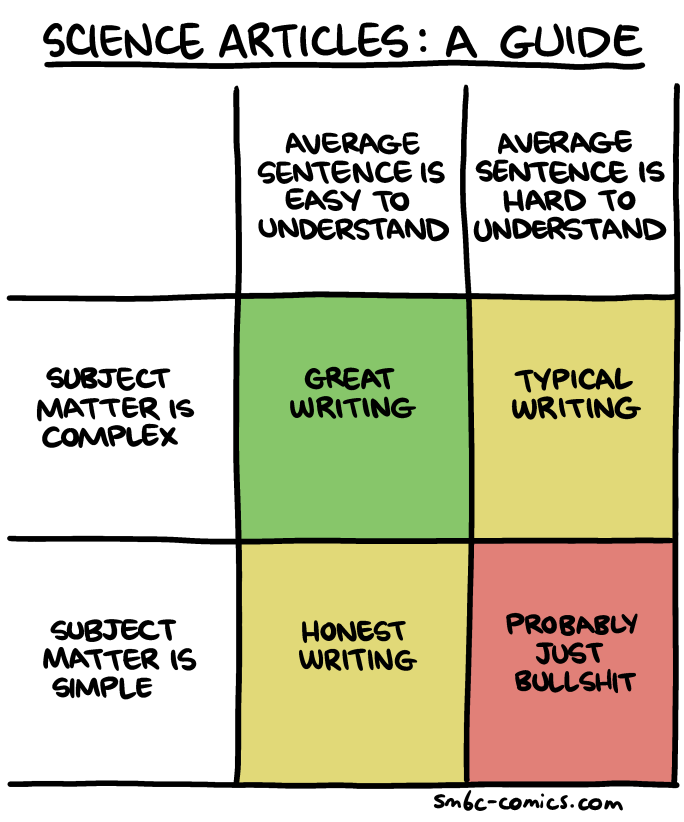
\includegraphics[width=0.55\textwidth]{science-articles-writing}
    \caption{Mouse-over text: ``All philosophy comics are off the chart, down and to the right.''}
    \label{fig:science-articles-writing}
\end{figure}

% Core theoretical ideas that make up your viewpoint. Includes: meaning of key concepts such as agency, learning, teaching, instruction, technology, skill, knowledge, etc.
\section{Kolb's experiential learning theory}
I'm pretty sold on the experiential learning theory (ELT) that David Kolb has propagated \citep{kolb2005kolb} and used as the basis for his learning styles inventory (LSI). This theory has its roots in Dewey, Lewin, Piaget, William James, Jung, Freire, Carl Rogers, and others. And yeah, I know that people freak out when we take different people's opinions and mash them together, but I think that's childish. This isn't theology where that's wrong. This is a different arena, one where we don't have absolute truth. There's so much overlap in these theories that it just makes sense to take a little from one and another little from another.

Some key points from Kolb's ELT are discussed in the following subsections.
\subsection{Learning is a process}
``Learning is best conceived as a process, not in terms of outcomes.'' I love this. Yes, I do care about the outcome, but I really care about the journey. It's all about the journey because that's how you get places.

\subsection{All learning is relearning}
``All learning is relearning.'' We must constantly be retaught things in order to truly learn them. There's a big reason the Lord repeats so often.

\subsection{Conflict drives learning}
``Conflict, differences, and disagreement are what drive the learning process.'' The times in my life that I have learned the most have come from having to argue something out. That's how things are proven. TODO: find a narrative from my life to fit this.

\subsection{Transactions between people and the environment}


\subsection{Process of creating knowledge}
``Learning is the process of creating knowledge.'' This is focusing on what I think is a semantic difference that we all just need to get over. This view is based on constructivism which says that a learner constructs new knowledge: ``social knowledge is created and recreated in the personal knowledge of the learner.'' It's contrasted to the transmission model whereby ``pre-existing fixed ideas are transmitted to the learner.'' This is purely semantic in my brain. Maybe I'm just too technical and not philosophical enough, but if knowledge is transmitted to the learner, the learner still has to construct that knowledge in their brain. I see learning like a child being given a new Lego set for Christmas: the Lego set is ``transmitted'' to the child, but the child must then ``construct'' the set into a final product. Constructing the product is what learning is all about. Mistakes will be made. The child might even have to rebuild the set a few times to really get it down.

(That might be getting a little complex for this metaphor. That's the idea that once we have learned new concepts, we must then deconstruct and reconstruct our previous knowledge. It's true, it just might be a little complex for the metaphor.)

It's like learning to play the piano. My piano teacher growing up would always ask me if I had played or if I had practiced. I always said that I'd practiced because that's what I called it when I sat at the piano and played things, but there was an important difference she was emphasizing: playing is sitting down and playing through the song; practicing is going through a song and, when a struggle point is reached, playing it over and over again until it's no longer a struggle.

Much like the child building a Lego set, it's important to find weak points in the learning process and go over them again and again until the set or piece is completed.

We can then get into deeper areas like what ``complete'' even means. An 8th grader can have a perfect understanding of all things at the 8th grade level, but that is surely a far cry from having a perfect understanding of all things. I don't want to get theological about this, but what exactly is a ``perfect understanding''? (Again, I'm not sure where this is going. Figure it out or get rid of it.)

We have to be careful when we set learning outcomes because it can make students feel like that's all there is to know. In the IT~347 (computer networks) class that I have TA's for a few years now, every semester the students complain that we never really get anywhere in the class. The problem is that we have to spend an entire semester learning foundational principles and protocols before we can even begin to have the deeper, funner conversations. Those are almost entirely reserved for IT~529 (advanced networking) because the students have to know \emph{so much} before we can begin to have deeper conversations: the \emph{why} conversations. The problem, though, (at least partially) is that students see the learning outcomes and they reach them, but they haven't really reached anything yet because it's still all foundational. They need a bit more direction. (This thought started out good, but ended not so strong. I'm not sure what I'm trying to prove here. Figure it out or get rid of it.)

% References from the scholarly literature (including from class) to situate your viewpoint in the world of ideas and help support your claims.
\bibliography{references}

\end{document}

Usually has the following features:
- Clearly identified audience/context at the beginning
- Modest scope: don't try to take on too much (less is more)
- Important assertions clarified and supported
- Smooth flow, coherent organization. Often with section headings.
